%%%%%%%%%%%%%%%%%%%%%%%%%%%%%%%%%%%%%%%%%%%%%%%%%%%%%%%%%%%%%%%%%%%%%%%%
% Plantilla TFG/TFM
% Universidad de Murcia. Facultad de Informática
% Realizado por: José Manuel Requena Plens
% Modificado: Pablo José Rocamora Zamora
% Contacto: pablojoserocamora@gmail.com
%%%%%%%%%%%%%%%%%%%%%%%%%%%%%%%%%%%%%%%%%%%%%%%%%%%%%%%%%%%%%%%%%%%%%%%%


\chapter{Resultados}

\section{Curva de ocupancia acumulada con proteína única}

El primer experimento mide exclusivamente la fase de inserción de proteínas, aislando el rendimiento del
algoritmo del resto de la cadena de PolNet. Se utiliza un único tipo de proteína (\texttt{2uv8\_10A},
dimensiones $48 \times 48 \times 48$ vóxeles) sobre el Tomograma 3, cuya membrana pre-existente ocupa
el $11.54\%$ del volumen. Los tres algoritmos (Tetris CPU, Tetris GPU y SAWLC) se ejecutan
secuencialmente sobre el mismo volumen y se registra la ocupancia total acumulada en función del tiempo
transcurrido.

\begin{figure}[H]
    \centering
    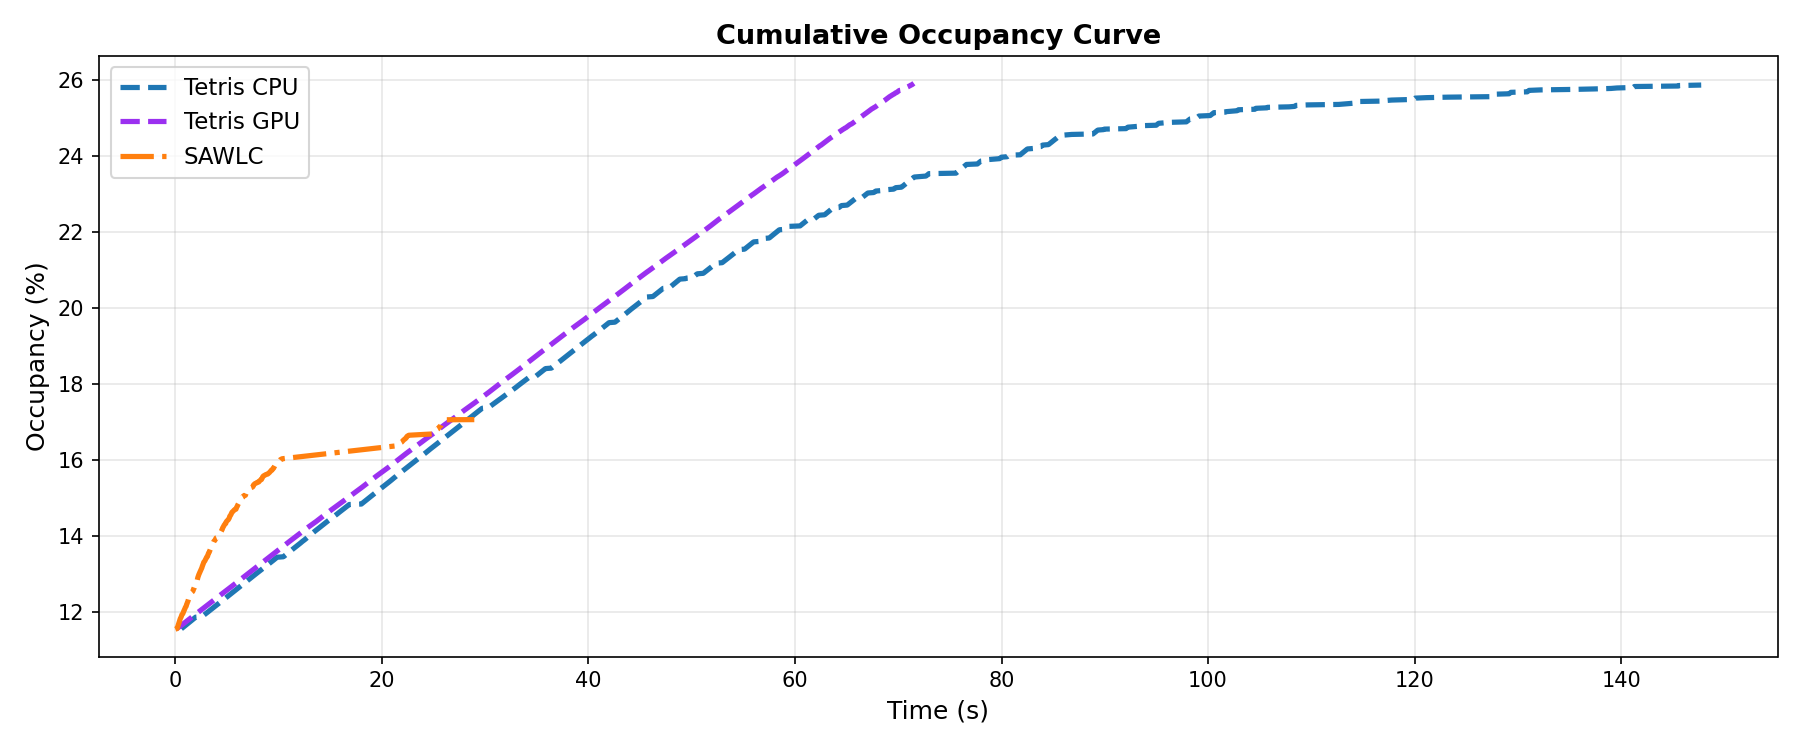
\includegraphics[width=1\textwidth]{archivos/profile_comparison-en.png}
    \caption{Curva de ocupancia acumulada en función del tiempo para los tres algoritmos evaluados
             sobre el Tomograma 3 con la proteína \texttt{2uv8\_10A}. El eje vertical parte del
             $11.5\%$ de la membrana; el incremento posterior corresponde íntegramente a proteínas
             insertadas.}
    \label{fig:profile-comparison}
\end{figure}

La Figura~\ref{fig:profile-comparison} muestra los resultados obtenidos. El eje Y parte del $\approx 11.5\%$
de ocupancia de la membrana, de modo que todo incremento posterior corresponde a proteínas insertadas.
Los resultados ponen de manifiesto tres comportamientos claramente diferenciados:

\begin{itemize}
    \item \textbf{SAWLC} (naranja) finaliza su ejecución en aproximadamente $25$\,s alcanzando una
    ocupancia total de $\approx 16.5\%$, lo que representa en torno a $5$ puntos porcentuales de
    proteína sobre la membrana. La detención temprana se debe a la fragmentación progresiva del espacio
    libre: la caminata aleatoria de SAWLC genera huecos intersticiales demasiado estrechos para alojar
    nuevos monómeros, por lo que el algoritmo agota sus intentos y se termina antes de saturar el volumen.

    \item \textbf{Tetris GPU} (morado) alcanza una ocupancia final de $\approx 25.8\%$ en $\approx 70$\,s.
    La guía por correlación FFT permite al algoritmo identificar y ocupar posiciones de contacto óptimas
    en el espacio libre residual, logrando una densidad de empaquetamiento casi tres veces superior a la
    de SAWLC.

    \item \textbf{Tetris CPU} (azul) converge al mismo techo de ocupancia ($\approx 25.8\%$) que la
    variante GPU pero requiere $\approx 145$\,s, lo que corresponde a un \textit{speedup} de $\approx
    \times 2.1$ del GPU sobre el CPU en este experimento de proteína única.
\end{itemize}

Estos resultados confirman que la estrategia de colocación guiada por FFT de Tetris es capaz de llenar
el volumen de forma significativamente más densa que SAWLC, y que la aceleración GPU reduce el tiempo de
ejecución sin alterar la ocupancia final alcanzada.

\section{Comparativa sistemática en el espectro completo de densidad}

El segundo experimento evalúa ambos algoritmos (Tetris en su variante GPU) a lo largo de un rango amplio
de densidades objetivo. Se define un barrido de \textit{targets} de ocupancia desde el $2.5\%$ hasta el
$57.5\%$ en pasos de $2.5\%$, lo que produce $23$ puntos de evaluación. Para obtener estimaciones
estadísticamente fiables, cada punto se repite \textbf{4 veces}, de modo que las curvas muestran la
media y la desviación típica de las ejecuciones. El experimento utiliza las 11 proteínas del conjunto de
pruebas sobre un tomograma vacío de $500 \times 500 \times 250$ vóxeles.

\begin{figure}[H]
    \centering
    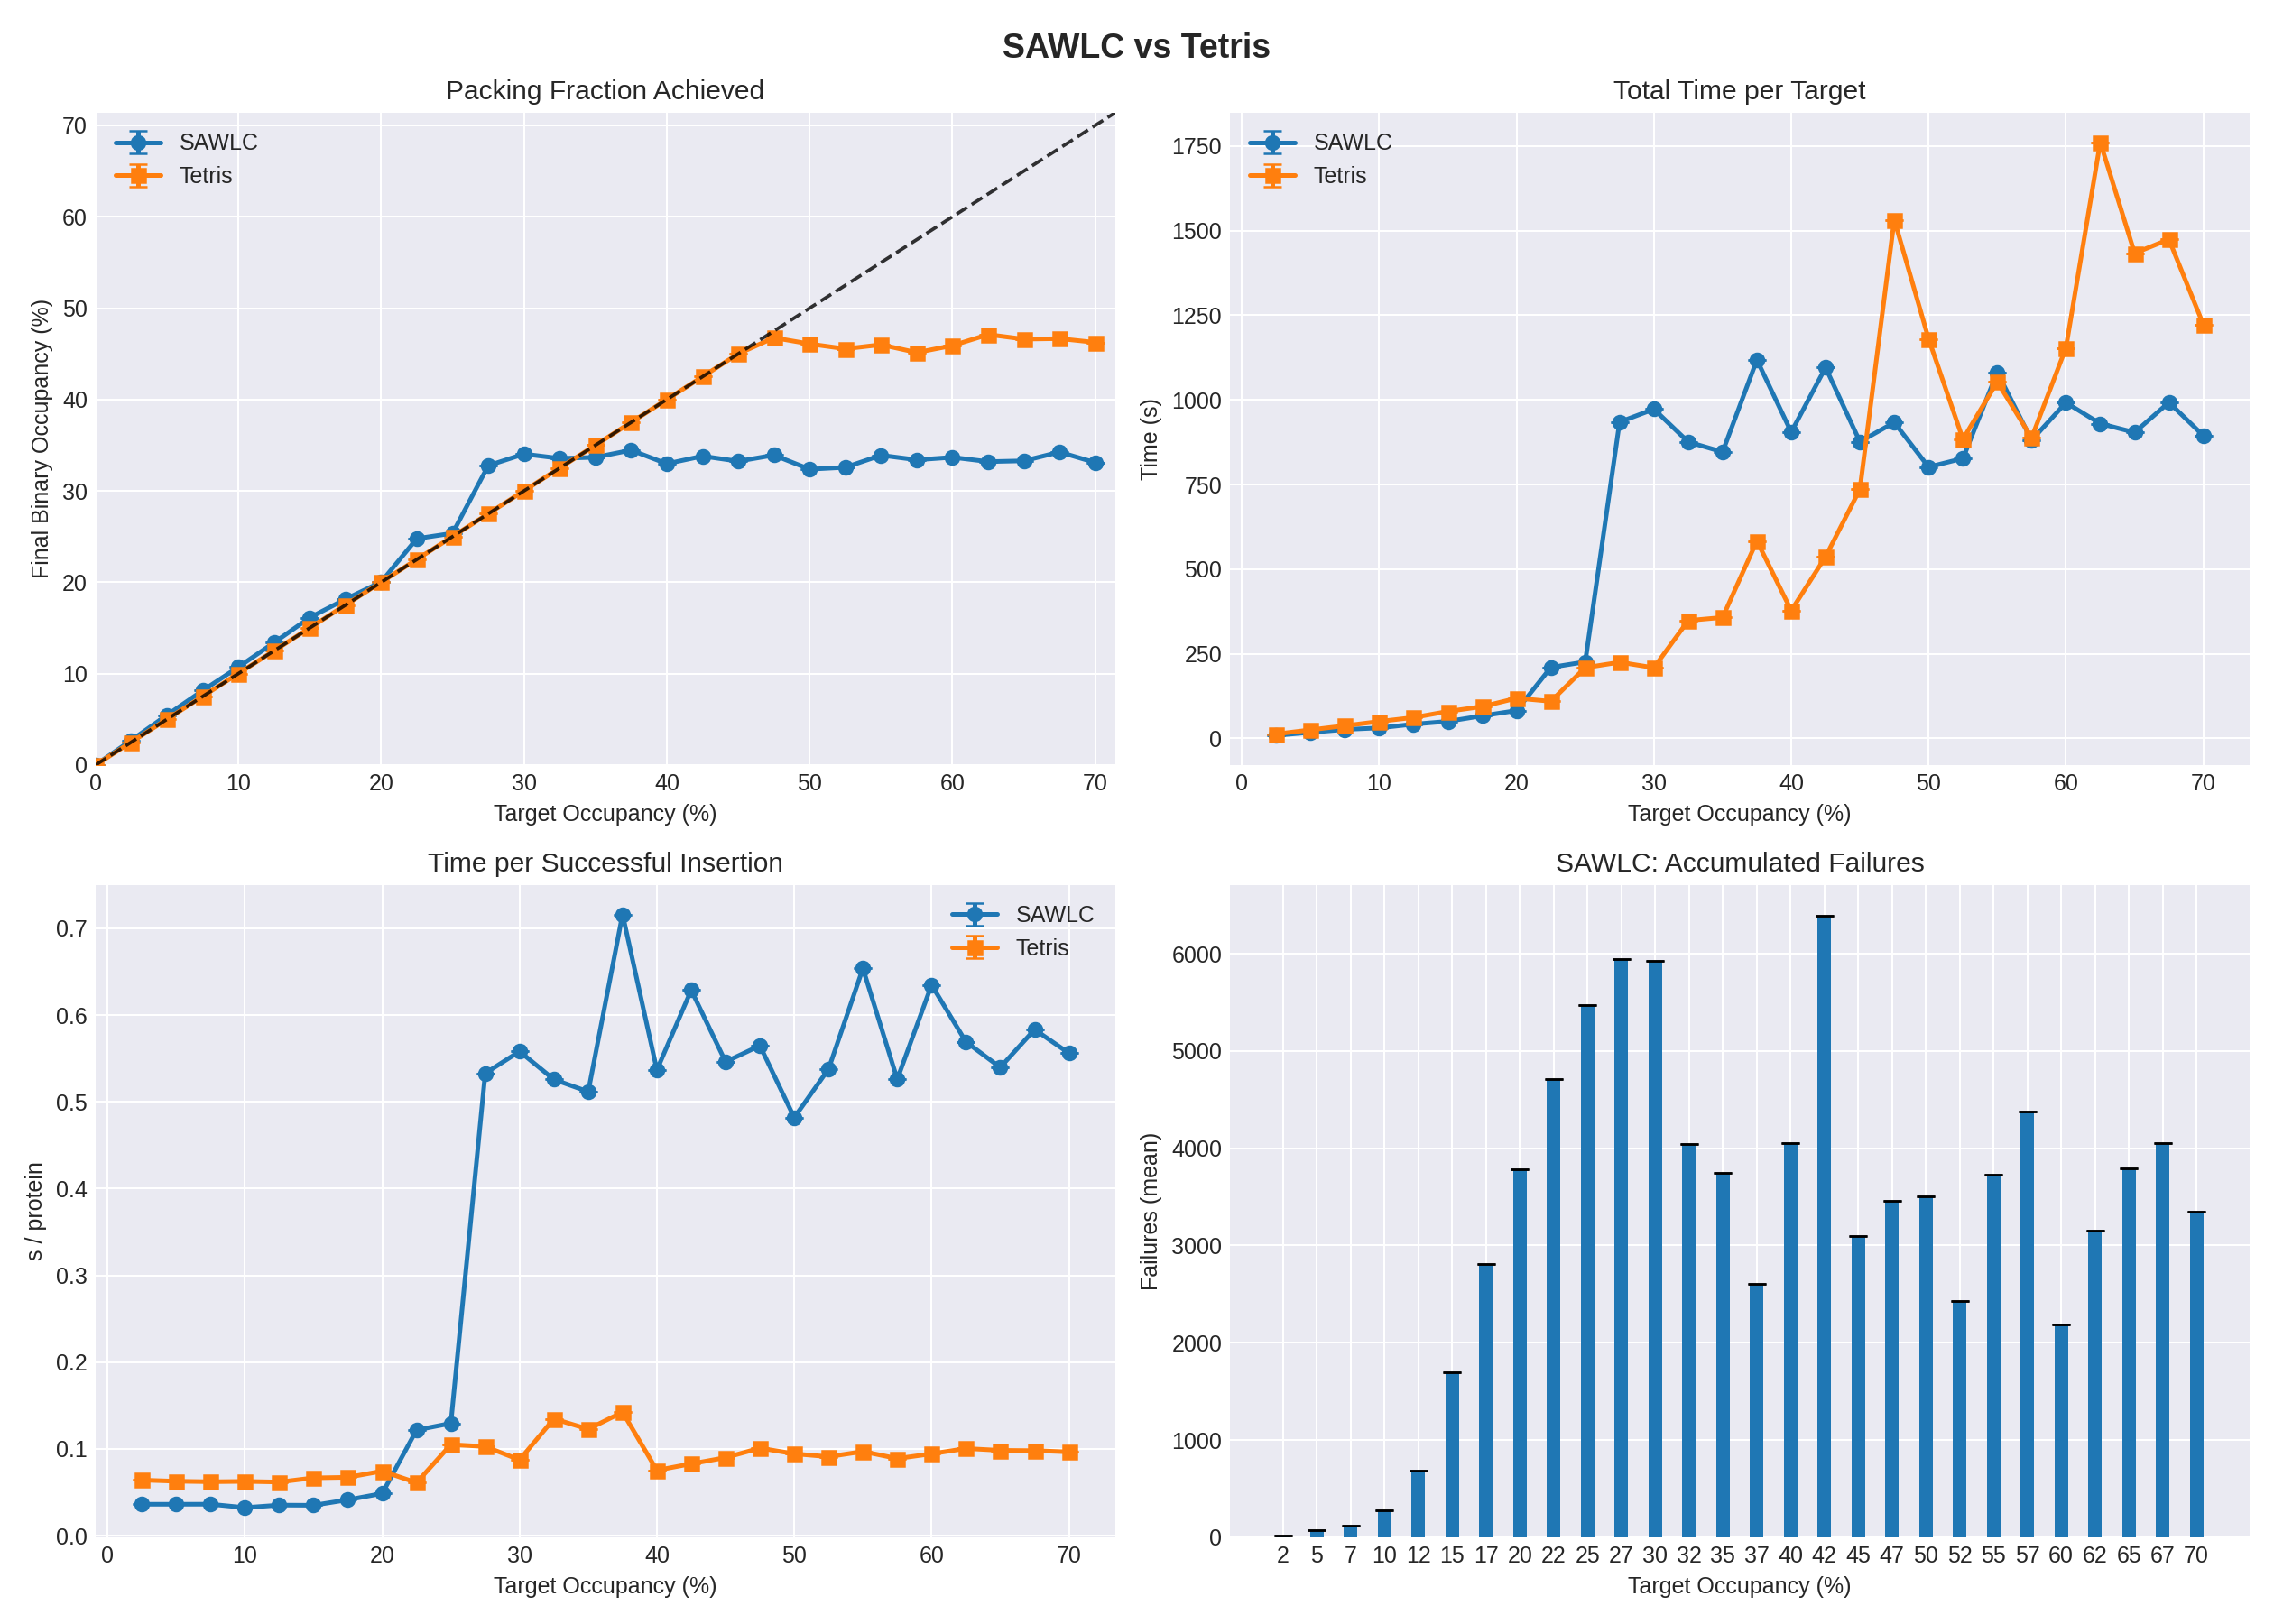
\includegraphics[width=1\textwidth]{archivos/benchmark_scientific_plots.png}
    \caption{Comparativa de ocupancia Tetris y SAWLC a lo largo del espectro completo de densidades
             objetivo. Cada punto representa la media de 4 repeticiones independientes con las 11
             proteínas del conjunto de pruebas.}
    \label{fig:benchmark-scientific}
\end{figure}

La Figura~\ref{fig:benchmark-scientific} agrupa cuatro subgráficas que analizan aspectos complementarios
del rendimiento de ambos algoritmos:

\begin{itemize}
    \item \textbf{Packing Fraction Achieved} (arriba izquierda). Representa la ocupancia final
    obtenida en función del target solicitado. La línea diagonal discontinua marca el ideal de ocupancia
    perfecta ($\text{obtenido} = \text{target}$); cuanto más se acerque una curva a esa diagonal, mayor
    es la capacidad del algoritmo de cumplir el objetivo de densidad.

    \item \textbf{Total Time per Target} (arriba derecha). Muestra el tiempo total de ejecución en
    segundos necesario para que cada algoritmo alcance (o intente alcanzar) el target indicado. Permite
    caracterizar el coste temporal de ambos algoritmos en función de la densidad solicitada.

    \item \textbf{Time per Successful Insertion} (abajo izquierda). Recoge el tiempo medio invertido
    por el algoritmo en insertar un único monómero con éxito, en segundos por proteína. Esta métrica
    refleja la eficiencia intrínseca de cada paso de inserción independientemente del número total de
    monómeros colocados.

    \item \textbf{SAWLC: Accumulated Failures} (abajo derecha). Muestra el número medio acumulado de
    intentos de inserción fallidos de SAWLC antes de que el algoritmo se detenga. Un fallo ocurre cuando
    una semilla candidata es rechazada por solapamiento o por estar fuera de los límites permitidos. Esta
    subgráfica se presenta únicamente para SAWLC porque Tetris, pese a disponer también de un parámetro
    de control de fallos consecutivos (\texttt{TRIES\_CLUSTERING}, con un umbral de 10 intentos), este
    número de fallos no se compara con el que produce SAWLC.
\end{itemize}

\section{Ocupancia máxima en función de la diversidad molecular}

El tercer experimento evalúa cómo evoluciona la ocupancia máxima alcanzable a medida que se incorporan
progresivamente más tipos de proteína. Se diseñan 11 pruebas acumulativas: la primera emplea únicamente
la proteína más grande del conjunto (\texttt{2uv8}), la segunda añade la siguiente en tamaño
(\texttt{5mrc}), y así sucesivamente hasta la prueba 11, en la que se utilizan los 11 tipos de proteína
simultáneamente. En cada prueba los algoritmos corren hasta agotar el volumen disponible sin imponer
ningún target de ocupancia. El tomograma de referencia contiene una membrana pre-existente que ocupa el
$11.5\%$ del volumen (línea discontinua en la Figura~\ref{fig:comparativa-completa}).

\begin{figure}[H]
    \centering
    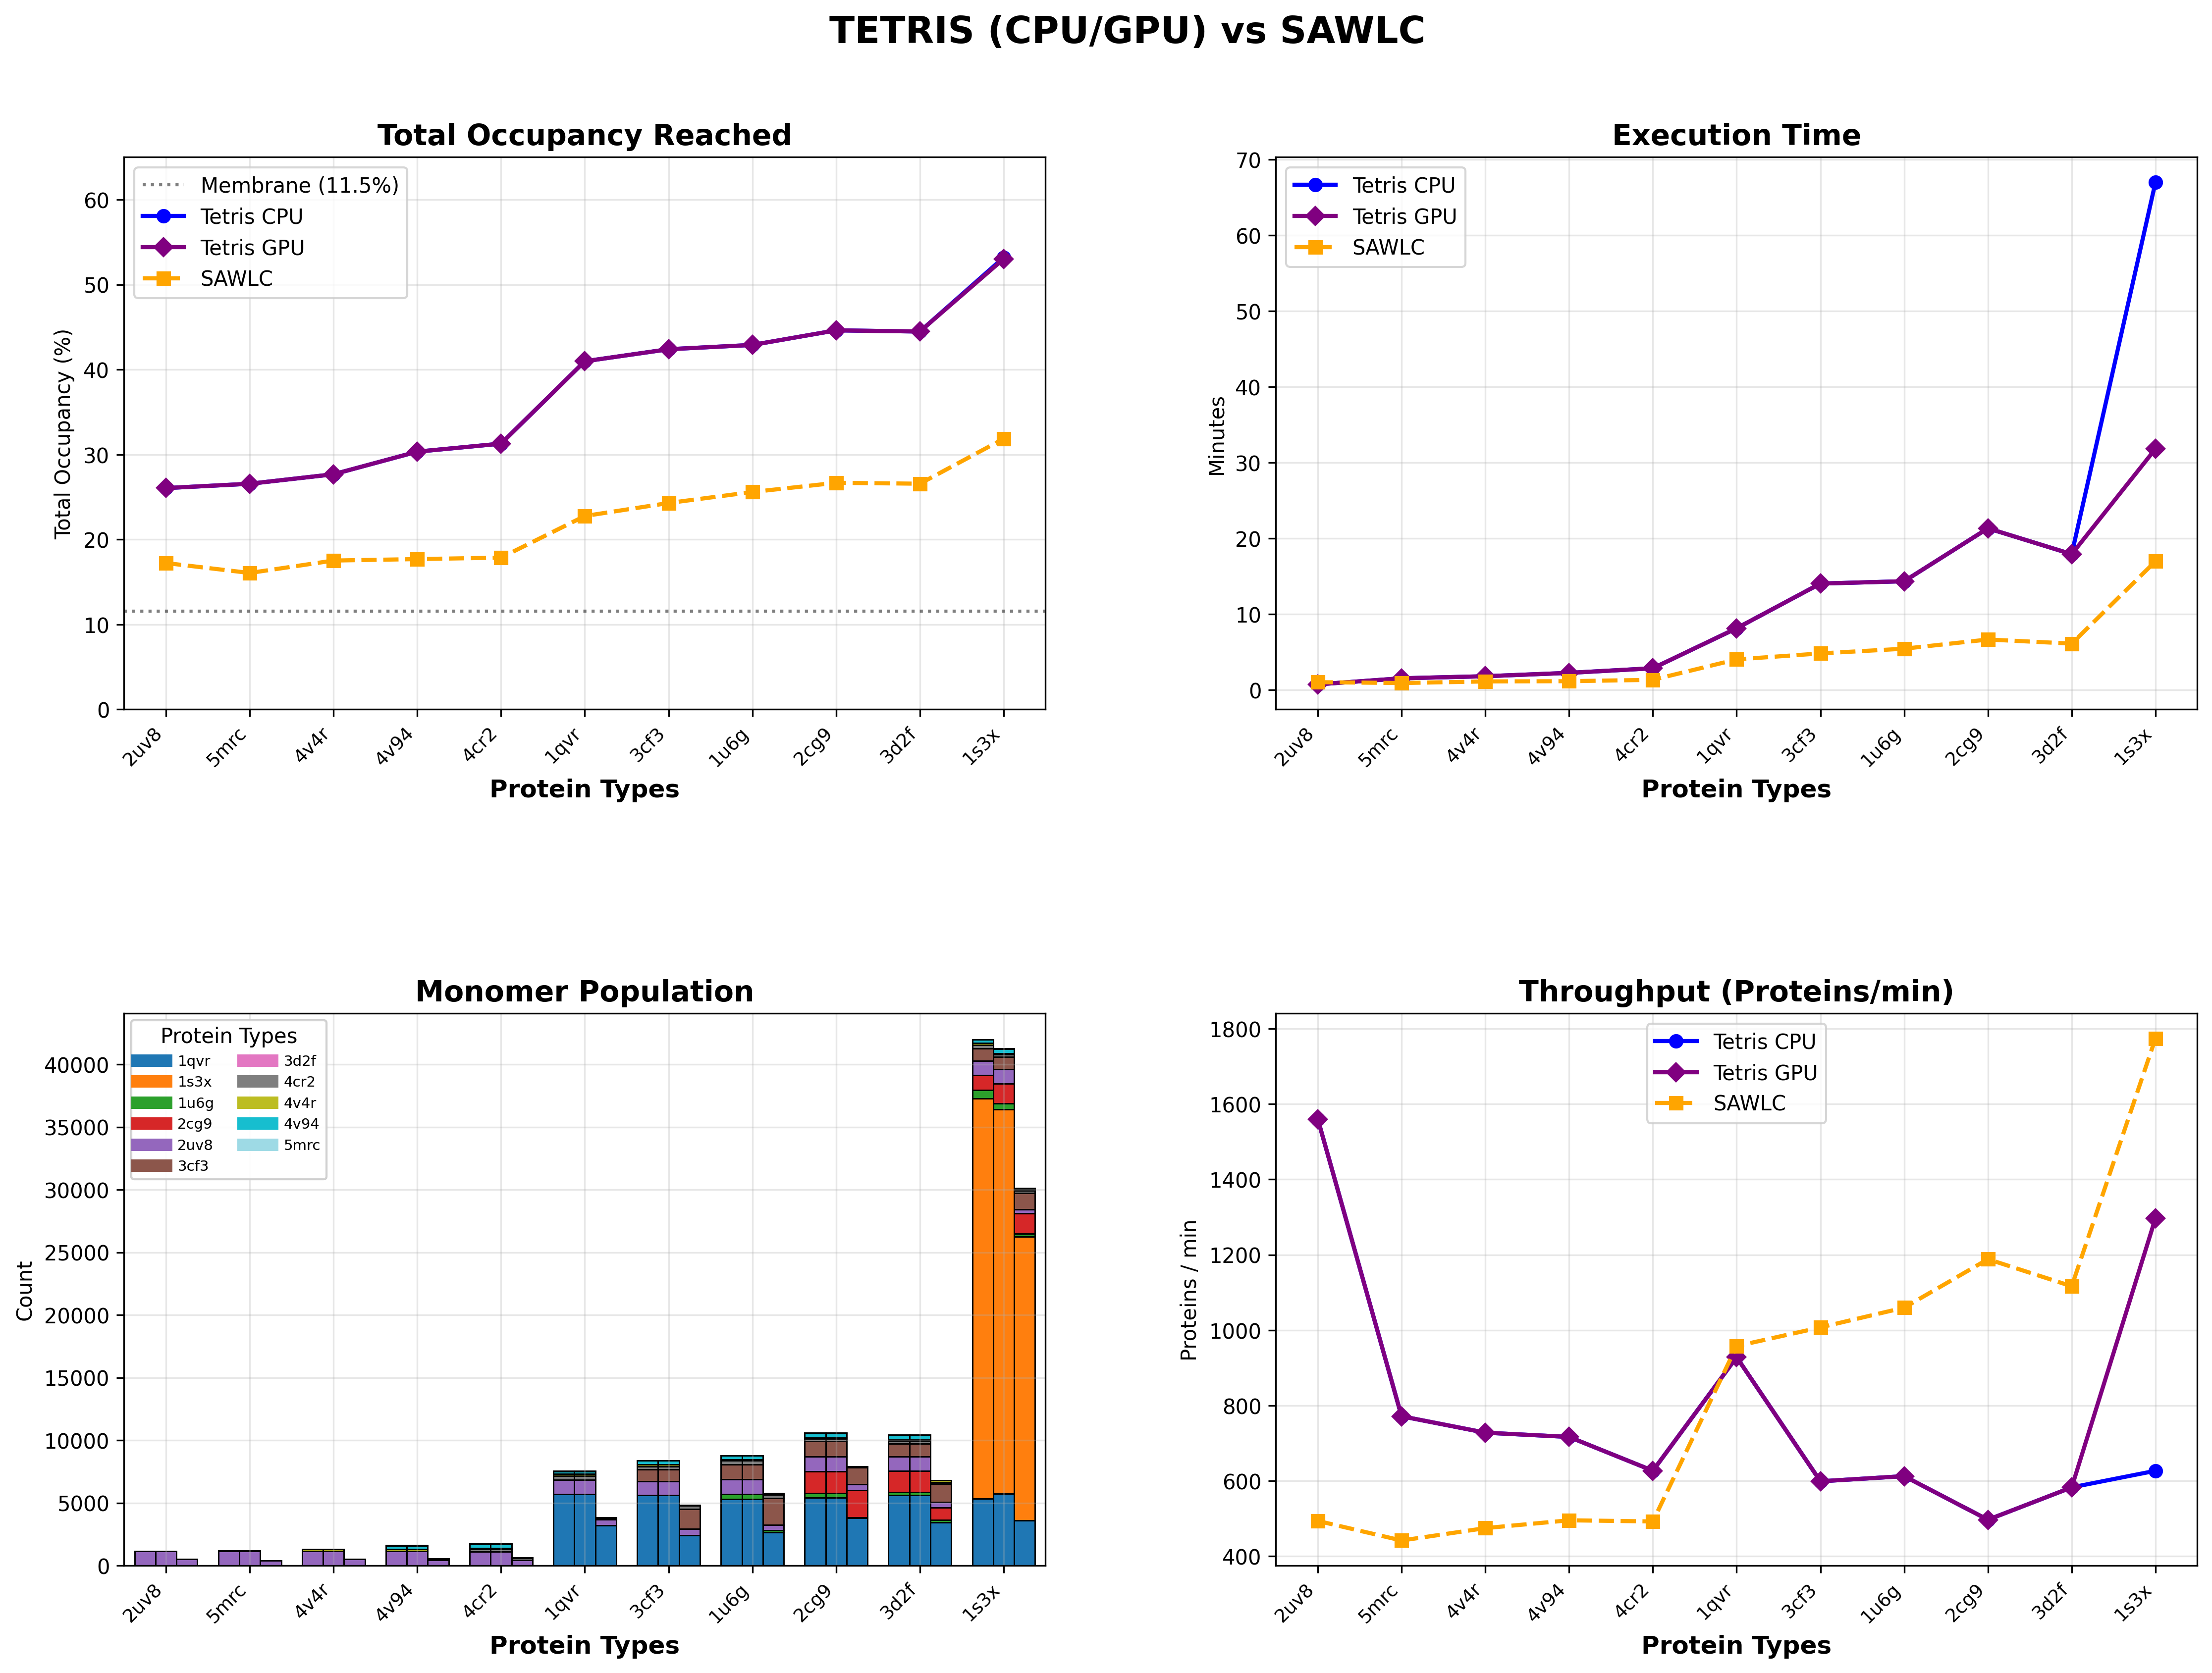
\includegraphics[width=1\textwidth]{archivos/resultados_comparativa_completa.png}
    \caption{Comparativa de Tetris (CPU/GPU) y SAWLC en función del número de tipos de proteína activos.
             Cada punto corresponde a una ejecución hasta saturación sobre el Tomograma 3.}
    \label{fig:comparativa-completa}
\end{figure}

Los resultados de la Figura~\ref{fig:comparativa-completa} muestran un patrón consistente a lo largo
de las cuatro subgráficas. En términos de ocupancia total alcanzada, SAWLC es el algoritmo más rápido
en tiempo de ejecución pero el que menor densidad de empaquetamiento consigue: su caminata aleatoria
satura pronto y deja una fracción significativa del volumen libre sin explotar. Tetris, en cambio,
aprovecha esa capacidad residual gracias a la guía por correlación FFT, lo que se traduce en una
ocupancia total notablemente superior en todas las combinaciones de proteínas. La variante GPU de Tetris
destaca especialmente: con los 11 tipos de proteína activos alcanza una ocupancia total de
aproximadamente el $52\%$ en torno a media hora de ejecución, lo que la convierte en la opción más
equilibrada entre densidad y coste temporal. La variante CPU logra valores de ocupancia similares a los
de la GPU, aunque con tiempos de ejecución sensiblemente mayores.

En cuanto a la población de monómeros, las barras apiladas reflejan que la mayor parte de las
inserciones corresponde a las proteínas de menor tamaño: al ocupar menos volumen individualmente,
pueden llenar los huecos intersticiales que las proteínas grandes dejan libres, contribuyendo de forma
decisiva al incremento de ocupancia total. Finalmente, el panel de throughput muestra que Tetris GPU
mantiene el mayor rendimiento sostenido a lo largo del experimento. SAWLC, por su parte, presenta un
throughput moderado en las primeras pruebas pero registra un pico muy pronunciado al incorporar
\texttt{1s3x}: al poder insertar miles de monómeros diminutos con gran rapidez mediante su caminata
aleatoria, supera puntualmente a Tetris GPU en este último punto. Tetris CPU mantiene el throughput más
bajo de los tres algoritmos de forma consistente.